\documentclass[11pt, letterpaper, onecolumn]{article}

\usepackage[english]{babel}
\usepackage{soul}
\usepackage{mathtools}
\usepackage[utf8]{inputenc}
\usepackage{graphicx}
\usepackage{float}
\usepackage[german=quotes]{csquotes}
\usepackage{hyperref}
\usepackage{fancyhdr}
\usepackage{gensymb}
\usepackage{units}
\usepackage{hhline}
\usepackage{color}
\usepackage{titling}
\usepackage[normalem]{ulem}
\usepackage[margin=2.5cm]{geometry}
\usepackage{amsmath}
\usepackage{amssymb}
\usepackage{amsfonts}
\usepackage{pgfplots}
\usepackage{array}
\usepackage{makecell}
\usepackage{subfigure}
\usepackage{lipsum}
\usepackage{url}
\usepackage{relsize}

\newgeometry{a4paper, left=20mm, right=20mm, top=30mm, bottom=30mm}
\definecolor{pantone294}{cmyk}{1,0.6,0,0.2}
\setlength{\columnsep}{6mm} 

\title{Project 1: QM point particle in external potential} 
\author{Florian Telleis / Florian Hollants / Mickey Wilke}
\date{\today}

\pagestyle{fancy}
\lfoot{Humboldt-Universität zu Berlin}
\rfoot{Project 1.1} 



\begin{document}
	
		Deckblatt: Revision 1.1 + Sub-project 1.2 
		
		\newpage
	
	
	
	
	
	
	\tableofcontents
	
	
	
	
	
	\vspace{0.5cm}
	
	
	\section{What changed regarding our first submission}
	
	\subsection{Modularity}
	As a first step, we improved our file management by implementing a modularity of files, dividing our prior one python file into seven (and of course more files for the second sub-project). The content of these modules did not change if not stated otherwise in the sections Variables, Tests or Convergence. \\
	The new file system is listed below: \\ 
	- "variables.py": defining variables and few general functions\\
	- "hamiltonian.py": defining potential and hamiltonian\\
	- "test$\_$hamiltonian.py": defining the tests for the hamiltonian and also running them for multiple $N$ and dimensions \\
	- "integrators.py": defining both the integrators \\
	- "test$\_$integrators.py": defining the tests for the integrators and also running them for multiple $N$ and dimensions \\
	- "test$\_$integr$\_$converg.py": testing the dependence of the integrators on $M$ or rather $\tau$ \\
	- "animation.py": defining functions for animation and animating


\subsection{Variables}
	We then changed/deleted all our old variables depending on other parameters to be now only defined by dimensionless values, without changing their value in regards to our first submission.
	In our case of modularity where we work with the same variables in multiple python files it is also practical to add an extra python file for storing our constant variables (and some basic functions used in multiple other files). We can then import these global variables by "from variables import *". \\
	This change worked with most of the prior functions and tests except when needing to change certain variables of a function in a separate file from where the function is defined. Explicitly, what changed: \\
	\textbf{1.} For the new hamiltonian tests (see 1.3), we had to change our definition of the potential to take $N$ from the size of the given array instead of using the global $N$.\\
	\textbf{2.} A second change regarding the hamiltonian file was done. We defined potential$\_$variable and \\hamilton$\_$variable which are the same as our old potential and hamiltonian but take $\mu$ and $\epsilon$ as an input for the convergence of eigenvalues/-vectors in the second sub-project. \\
	\textbf{3.} Similarly, but for the first sub-project, for testing the integrators in dependence of $M$ or rather $\tau$, we had to add an additional input for $\tau$ into the integrators (and therefore the tests). Therefore, the dependence could be evaluated without having to define the integrators in the same file as the tests, which was done in our first submission.


	\subsection{Tests}
	The tests we included in the sub-project 1 were in general not modified for this revision. We now ran these tests of the hamiltonian and integrators for multiple dimensions and $N$ for proper testing. Here we take focus on $N$ = 5, 10, 15 and 20; because the relevance of boundary conditions and resulting errors decrease for large $N$. The exact output for running the testing files is shown in the following figures for each of the $N$ for 4 dimensions (hamiltonian) and 3 dimensions (integrators, due to long run-time). The tests are including "randomly" generated arrays. Therefore these tests run 10 times each and depending on the criteria the maximum error of each test is saved.\\
	Also notice that the output shows $N$ as a float, it is an integer nonetheless.
	\begin{figure} [h] 
	\begin{center}
	\includegraphics[width=15cm]{"test_hamiltonian2.png"}
	\caption{Output of our test functions for the hamiltonian for multiple $N$ and $D$; 10 iterations.}
	\end{center}
	\end{figure}
	\\
	One can see that the errors for testing the linearity and eigenvectors are in the range of $10^{-14}$ to $10^{-13}$, where for higher dimensions the error increases. It also seems that for higher $N$ the errors also increase. But in some cases this could also be due to the "random" generation. We observe the same dependence for the hermiticity with errors up to $10^{-10}$ and eigenvectors with error up to $10^{-12}$. The positivity of the hamiltonian was correct all the iterations.\\
	\\
	Now our integrator tests. 
	\begin{figure} [h] 
	\begin{center}
	\includegraphics[width=13cm]{"test_integrators2.png"}
	\caption{Output of our test functions for the integrators for multiple $N$ and $D$; 10 iterations.}
	\end{center}
	\end{figure}
	\\
	The errors of unitarity for the strang-splitting integrator and linearity for both of the integrators are in the range of $10^{-16}-10^{-15}$, which is even smaller than for the hamiltonian tests and checks with the expectation. The unitarity errors for the second-order integrator are far larger even in 1D with $10^{-5}$ and rising for higher dimensions. Even greater errors can be seen for the energy conservation tests. This is expected as energy conservation is not given for these integrators. The important detail however, is that no significant lowering of errors for higher $N$ is seen, which is most likely due $N=20$ still being relatively small and using randomly generated arrays, which change the error maxima.
	\\
	\\
	Below, all the tests were run for one iteration for $N=5$ and $D=9$ as an additional testing. One can see the same behaviour as above, just exaggerated. \\
	With all these evaluated results we can safely conclude that our tests run (correctly) in more dimensions than $D=1$, even for small $N$.
	\begin{figure} [h] 
	\begin{center}
	\includegraphics[width=6cm]{"test_hamiltonian-9D2.png"}
	\caption{Output of our test functions for the hamiltonian for $N=5$ and $D=9$; 1 iteration.}
	\end{center}
	\end{figure}
	\begin{figure} [h] 
	\begin{center}
	\includegraphics[width=7cm]{"test_integrators-9D2.png"}
	\caption{Output of our test functions for the integrators for $N=5$ and $D=9$; 1 iteration.}
	\end{center}
	\end{figure}
	
	
	
	
	
	
	
	\subsection{Convergence with rel() function xxxxxxxchange title}
	- Flo H
	
	

	\\
 	\\
  	\\
   	\\
 	(noch die neue Animation reinpacken um zu zeigen dass modular funktioniert?)
  	\\
   	\\
    	\\
	
	\section{How the code works for the second sub-project}	
	
	
	
	
	\section{Workflow}
	
	
	
	
	\section{Implementing conjugate-gradient and power method}
	
	
	
	
	\section{Testing}
	!!! describe this time with detail and test all possible configurations!!!
	
	
	
	\section{Convergence of eigenvalues/eigenvectors}

 	\subsection{Infinite Volume Limit}
  	We first try to do the infinite volume limit, by using the arnoldi-method for a random starting vector and a fixed value of $\mu=20$, $\varepsilon=\frac{1}{60}$ and $N=40$. Then we repeat that process for bigger values of $N$ and plot the eigenvalues against $N$.
    	\begin{figure} [h] 
	\begin{center}
	\includegraphics[width=7cm]{"inf_vol_lim.png"}
	\caption{Eigenvalues of the of the Hamiltonian for different values of $N$}
	\end{center}
	\end{figure}
	The eigenvectors seem to have converged from $N=200$ onwards although two of the four eigenvalues seem to have vanished. Zooming in on one the lower dot reveals, that the two eigenvalues are much closer compared to the distance to the other two eigenvalues. Since we don't expect the eigenvalues to change much anymore, we say that the infinite volume limit is well approximated for $N>240$. 
 	








%	\hyperref[Quellen]{$^{[1]}$}	



	
%		\begin{figure} [h] 
%	\begin{center}
%	\subfigure[CGM]{\includegraphics[width=0.45\textwidth]{799px-Constant_current.svg.png}}
%    \subfigure[CHM]{\includegraphics[width=0.45\textwidth]{799px-Constant_height.svg.png}}
%\caption{Verschiedene Modi für das RTM Abrastern, entnommen aus \hyperref[Quellen]{[3]}}
%	\end{center}
%	\end{figure}


	

	
	%	\begin{figure} [h] 
%	\begin{center}
%	\includegraphics[width=8.8cm]{"QBER(R).jpg"}
%	\caption{QBER($R_{det}$) for three different photon sources and different attenuations; the data points are linearly connected for better visibility}
%	\end{center}
%	\end{figure}
	
	
	

%	\hyperref[Quellen]{$^{[1]}$}	

	
	
\newpage
	

	
%\section{Sources and Literature} \label{sources}
%
%		$[1]$ \textit{Titel} - Autor; (Vers.) Datum
%\vspace{0.4cm}
%		 \\
%		$[2]$ Internetseite: \textit{Titel} \\ \url{Link} \\- zuletzt besucht am Datum um Zeit
%		\vspace{0.4cm}
%		 \\
		
		
%		$[1]$ \textit{Titel} - Autor; (Vers.) Datum
%\vspace{0.4cm}
%		 \\
%		$[2]$ Internetseite: \textit{Titel} \\ \url{Link} \\- zuletzt besucht am Datum um Zeit
%		\vspace{0.4cm}
%		 \\

	
	

	
\section{Appendix} \label{sec:appendix}

%	\begin{figure}[h]	
%	\begin{center}	
%	\subfigure[Random input wavefunction]{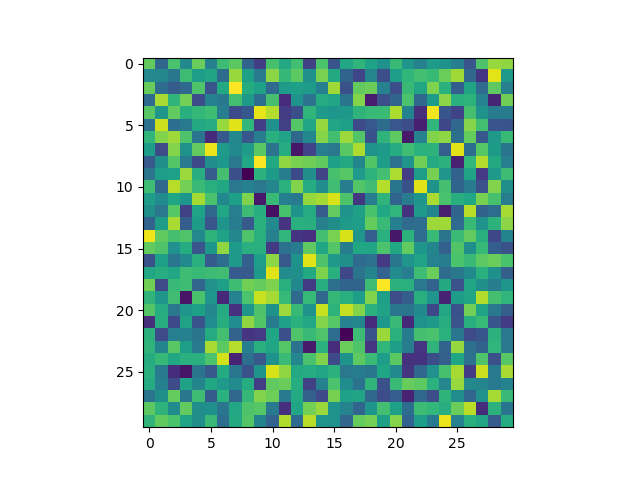
\includegraphics[width=0.35\textwidth]{function1_ABS.png}}
%    \subfigure[Potential]
%    {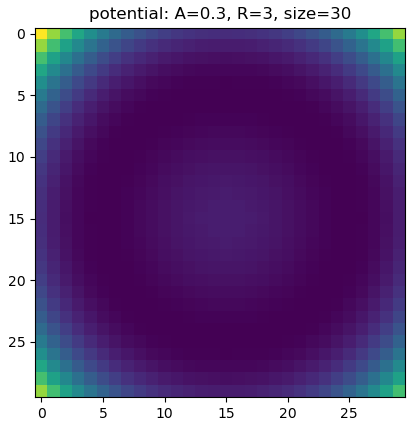
\includegraphics[width=0.35\textwidth]{potential2.png}}
%    \subfigure[Second-order integration]
%    {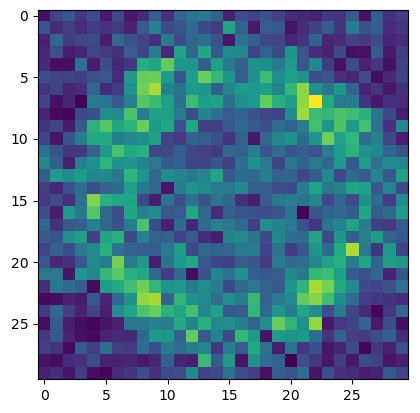
\includegraphics[width=0.35\textwidth]{so-integrator1_ABS.png}}
%	\caption{Tests with (a) random 2D wavefunction, (b) resulting potential and (c) the following time evolution with the second-order integrator after a certain amount of time steps M (not known anymore, but around 2000 with T=2)}
%	\label{fig:2D-so_integr}
%	\end{center} 
%	\end{figure}
	
	




	
\end{document}
